\chapter{Anhang}
\label{cha:anhang}

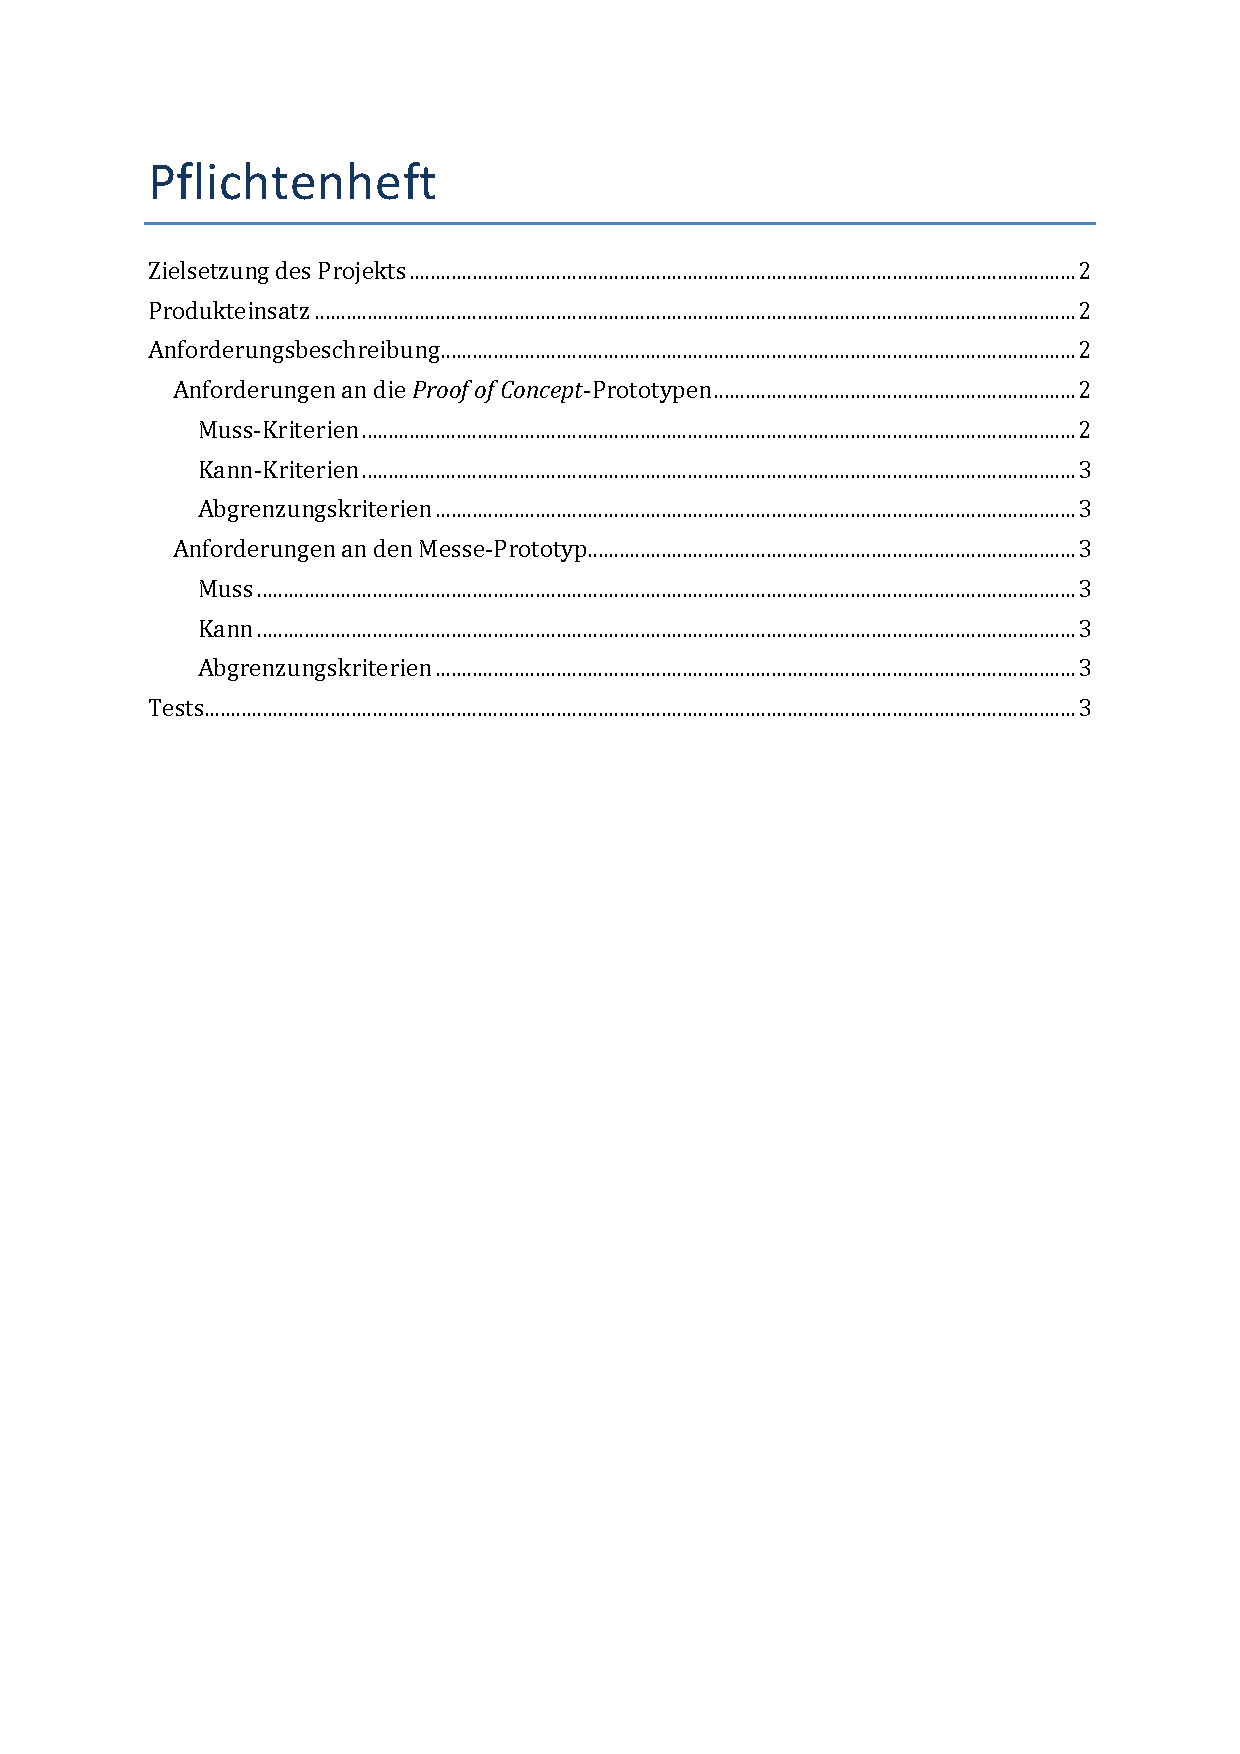
\includepdf[pages={-},frame= true, scale=0.68, pagecommand=\section{Pflichtenheft}\label{sec:Pflichtenheft}]{content/additional/Pflichtenheft.pdf}

\section{Cache Post}
\label{sec:cachePost}

%CachePush-Bild
\begin{figure}[!h]
\centering
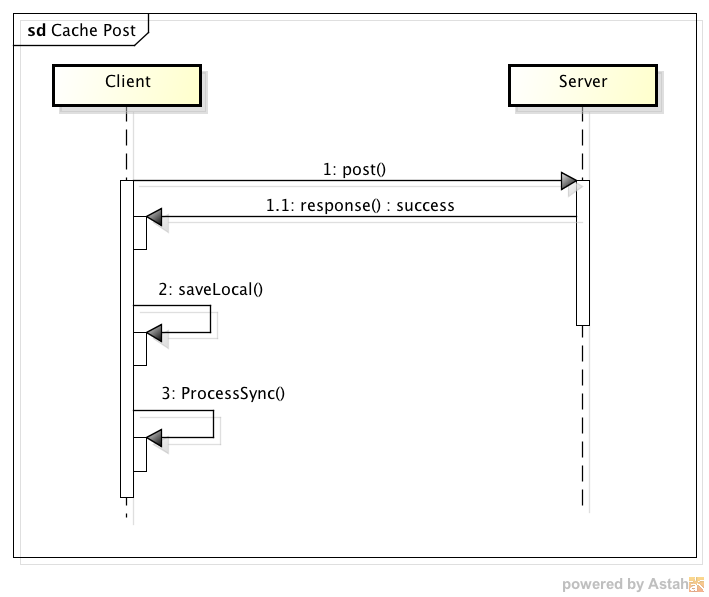
\includegraphics[width=0.8\linewidth]{content/images/Cache-Post}
\caption{Hochladen zum Server}
\label{pic:cachePost}
\end{figure}

\section{User-Story in der nativen App}
\label{sec:UserStory}
%Startseite
\begin{figure}[!h]
\centering
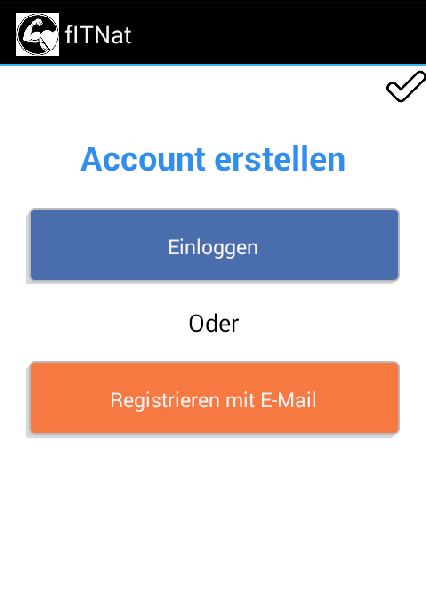
\includegraphics[width=0.5\linewidth]{content/images/App/Startseite}
\caption{Startseite}
\label{pic:natAppStartseite}
\end{figure}
%Login
\begin{figure}[!h]
\centering
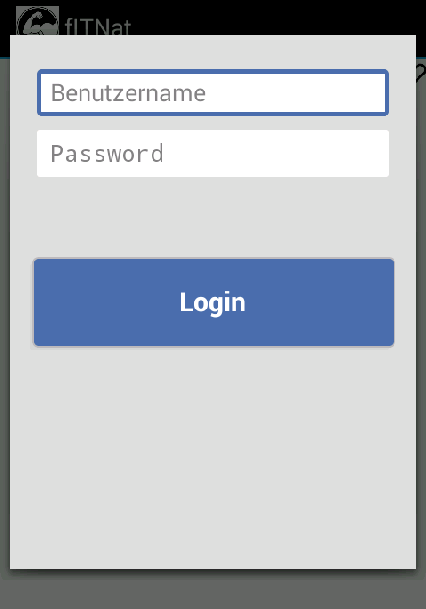
\includegraphics[width=0.5\linewidth]{content/images/App/SignIn}
\caption{Login}
\label{pic:natAppLogin}
\end{figure}
%Reistrierung
\begin{figure}[!h]
\centering
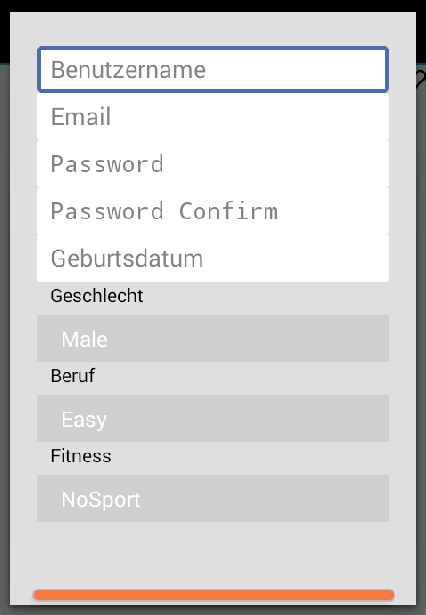
\includegraphics[width=0.5\linewidth]{content/images/App/SignUp}
\caption{Registrierung}
\label{pic:natAppRegistrierung}
\end{figure}
%Trainingspläne
\begin{figure}[!h]
\centering
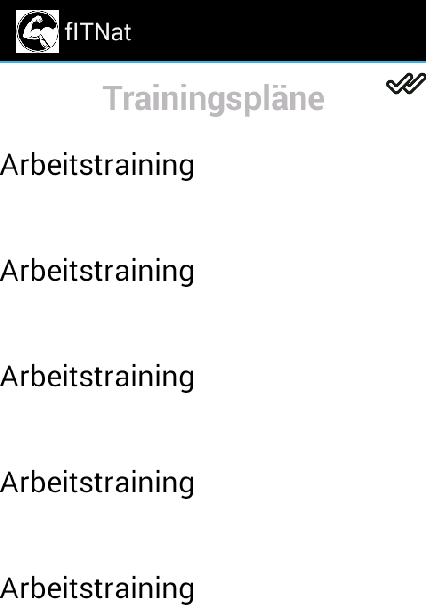
\includegraphics[width=0.5\linewidth]{content/images/App/Trainingsplan}
\caption{Übersicht der Trainingspläne}
\label{pic:natAppTrainingspläne}
\end{figure}
%Übungen
\begin{figure}[!h]
\centering
\includegraphics[width=0.5\linewidth]{content/images/App/Übungen}
\caption{Übersicht der Übungen}
\label{pic:natAppÜbungen}
\end{figure}
%Training
\begin{figure}[!h]
\centering
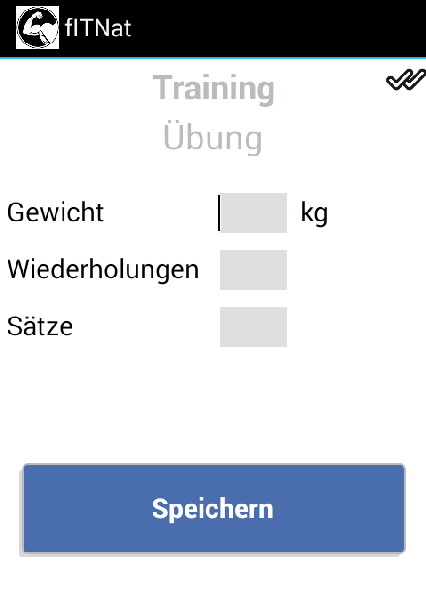
\includegraphics[width=0.5\linewidth]{content/images/App/Training}
\caption{Training}
\label{pic:natAppTraining}
\end{figure}
%Statistik
\begin{figure}[!h]
\centering
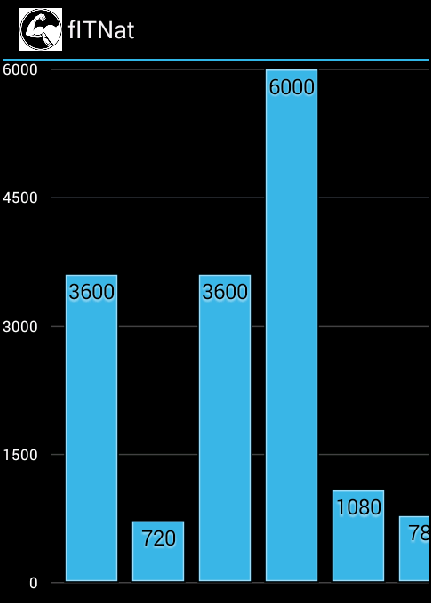
\includegraphics[width=0.5\linewidth]{content/images/App/Statistik}
\caption{Statistik}
\label{pic:natAppStatistik}
\end{figure}

\section{Funktionsumfang}
\label{natAppFunktionen}